%%%%%%%%%%%%%%%%%%%%%%%%%%%%%%%%%%%%%%%%%
% LaTeX Template
% http://www.LaTeXTemplates.com
%
% Original author:
% Linux and Unix Users Group at Virginia Tech Wiki 
% (https://vtluug.org/wiki/Example_LaTeX_chem_lab_report)
%
% License:
% CC BY-NC-SA 3.0 (http://creativecommons.org/licenses/by-nc-sa/3.0/)
%
%%%%%%%%%%%%%%%%%%%%%%%%%%%%%%%%%%%%%%%%%

%----------------------------------------------------------------------------------------
%	PACKAGES AND DOCUMENT CONFIGURATIONS
%----------------------------------------------------------------------------------------

\documentclass[12pt]{article}
\usepackage{geometry} % Pour passer au format A4
\geometry{hmargin=1cm, vmargin=1cm} % 

\usepackage{graphicx} % Required for including pictures
\usepackage{float} % 

%Français
\usepackage[T1]{fontenc} 
\usepackage[english,francais]{babel}
\usepackage[utf8]{inputenc}
\usepackage{eurosym}
\usepackage{lmodern}
\usepackage{url}
\usepackage{multicol}

%Maths
\usepackage{amsmath,amsfonts,amssymb,amsthm}
%\usepackage[linesnumbered, ruled, vlined]{algorithm2e}
%\SetAlFnt{\small\sffamily}

%Autres
\linespread{1} % Line spacing
\setlength\parindent{0pt} % Removes all indentation from paragraphs

\renewcommand{\labelenumi}{\alph{enumi}.} % 
\pagestyle{empty}
%----------------------------------------------------------------------------------------
%	DOCUMENT INFORMATION
%----------------------------------------------------------------------------------------
\begin{document}

%\maketitle % Insert the title, author and date

\setlength{\columnseprule}{1pt}

\textbf{Nom(s), Prénom(s) :}

\subsection*{1 - Équation de la chaleur}

\fbox{\begin{minipage}{\textwidth}
    On se propose de résoudre par étape le problème suivant.\\

    Un bloc de céramique initialement à 40 degré est mis dans dans un four dont la température constante est de 1000 degré. On suit la fonction $y$ qui dépend du temps $t$. La température du bloc est régit par l'équation suivante. 

    \begin{equation*}
      \left\lbrace
      \begin{array}{ccc}
        y'   &=& k(1000 - y) \text{ avec k une constante non nulle qui dépend du four.}\\
        y(0) &=& 40
      \end{array}\right.
    \end{equation*}

    On se propose de prendre un four avec un coefficient $k = 0.2$.
\end{minipage}}


\begin{enumerate}
\item Chercher l'ensemble des solutions $y_G$ de l'équation sans second membre.
  $$ y_G' + 0.2y_G = 0 $$
\item Vérifier que la fonction $y_p = 1000 + e^{-0.2t}$ est solution de l'équation avec second membre. 
  $$ y_p' = 0.2(1000 - y_p) $$
\item Soit $y$ la solution générale de notre problème initiale.
  \begin{equation*}
    \left\lbrace
    \begin{array}{ccc}
      y'   &=& 0.2(1000 - y)\\
      y(0) &=& 40
    \end{array}\right.
  \end{equation*}
  Après avoir écrit $y = y_G + y_p$, chercher l'unique solution vérifiant la condition initiale $y(0) = 40$. 
\item Tracer la fonction $y$ solution de ce problème.
\end{enumerate}

\begin{figure}[H]
  \centering
  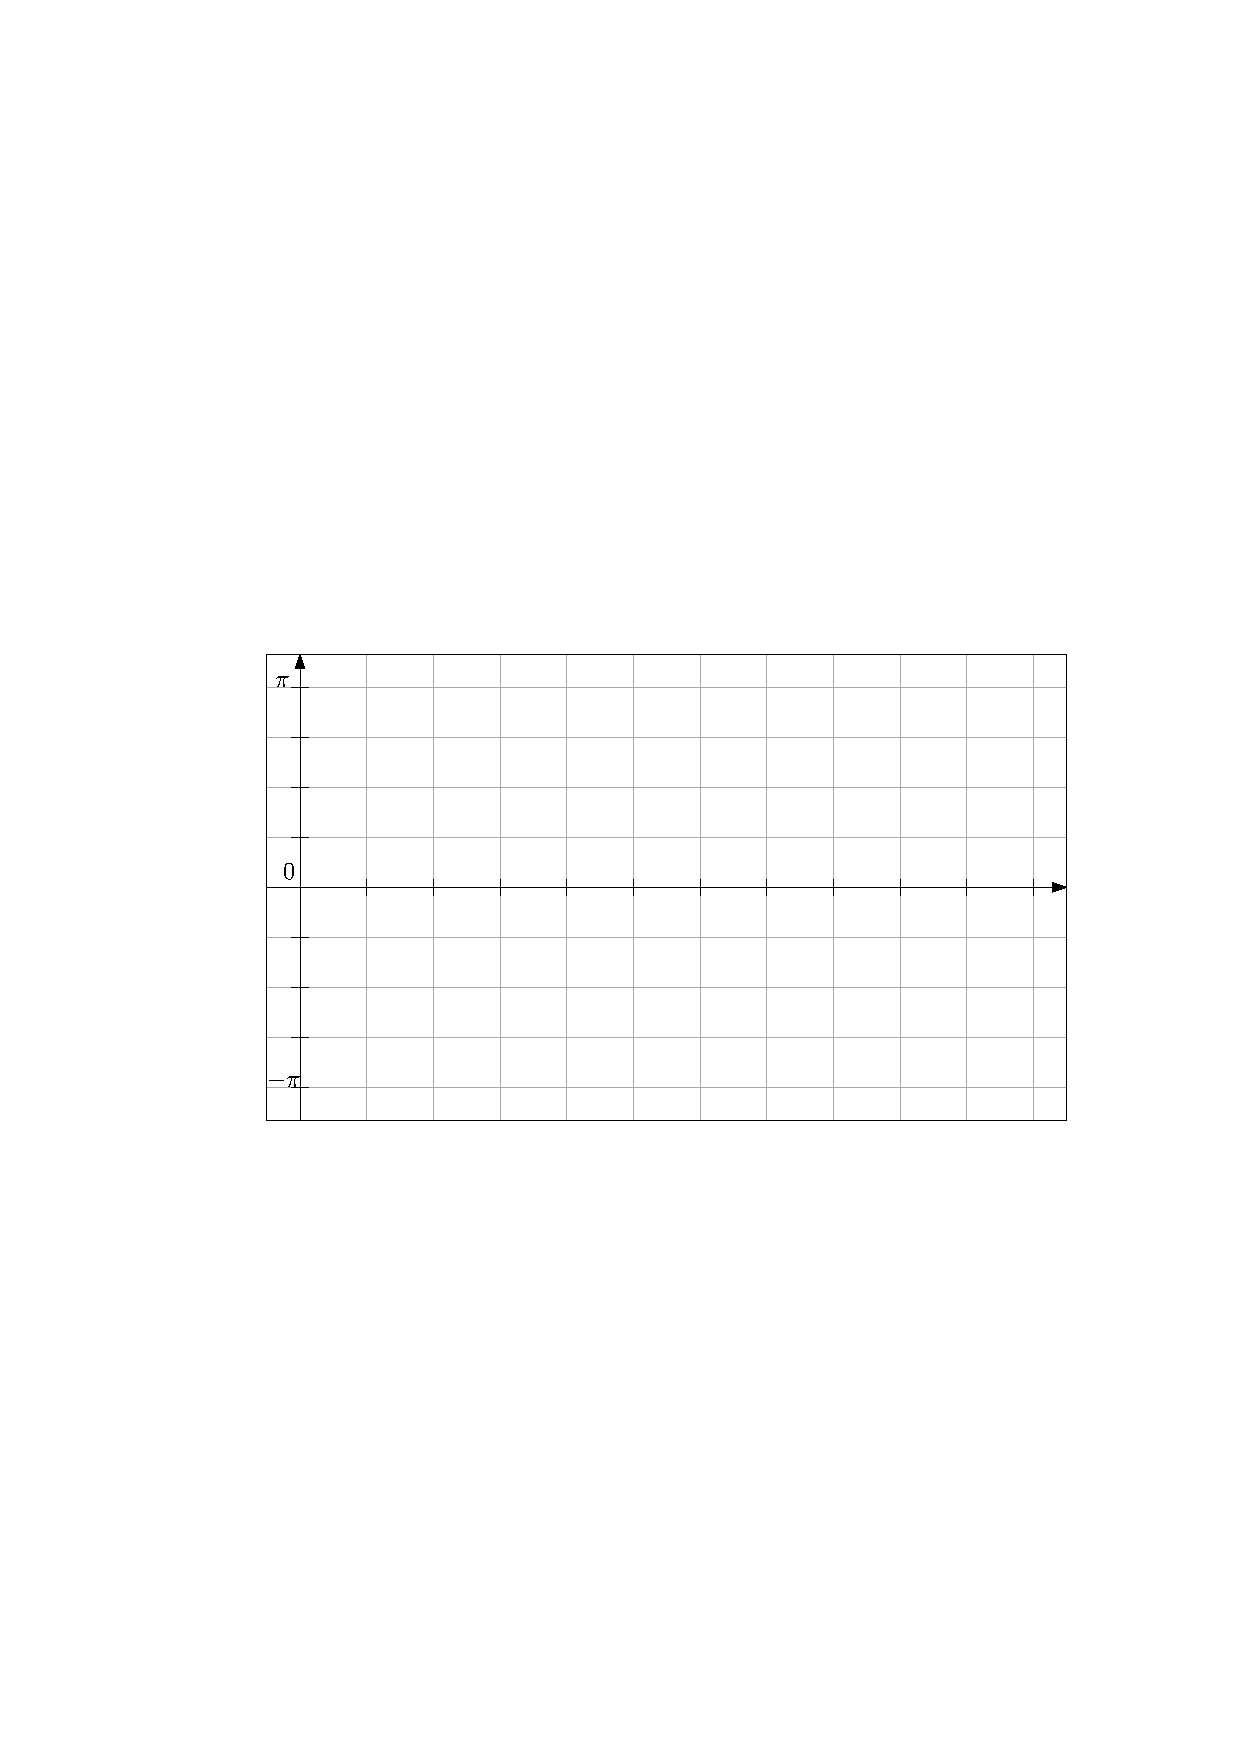
\includegraphics[width=\linewidth]{sources/1/grille.pdf}
\end{figure}

\newpage

\textbf{Nom(s), Prénom(s) :}

\subsection*{1 - Équation de la chaleur}

\fbox{\begin{minipage}{\textwidth}
    On se propose de résoudre par étape le problème suivant.\\

    Un bloc de céramique initialement à 40 degré est mis dans dans un four dont la température constante est de 1000 degré. On suit la fonction $y$ qui dépend du temps $t$. La température du bloc est régit par l'équation suivante. 

    \begin{equation*}
      \left\lbrace
      \begin{array}{ccc}
        y'   &=& k(1000 - y) \text{ avec k une constante non nulle qui dépend du four.}\\
        y(0) &=& 40
      \end{array}\right.
    \end{equation*}

    On se propose de prendre un four avec un coefficient $k = 0.2$.
\end{minipage}}


\begin{enumerate}
\item Chercher l'ensemble des solutions $y_G$ de l'équation sans second membre.
  $$ y_G' + 0.2y_G = 0 $$
\item Vérifier que la fonction $y_p = 1000 + e^{-0.2t}$ est solution de l'équation avec second membre. 
  $$ y_p' = 0.2(1000 - y_p) $$
\item Soit $y$ la solution générale de notre problème initiale.
  \begin{equation*}
    \left\lbrace
    \begin{array}{ccc}
      y'   &=& 0.2(1000 - y)\\
      y(0) &=& 40
    \end{array}\right.
  \end{equation*}
  Après avoir écrit $y = y_G + y_p$, chercher l'unique solution vérifiant la condition initiale $y(0) = 40$. 
\item Tracer la fonction $y$ solution de ce problème.
\end{enumerate}

\begin{figure}[H]
  \centering
  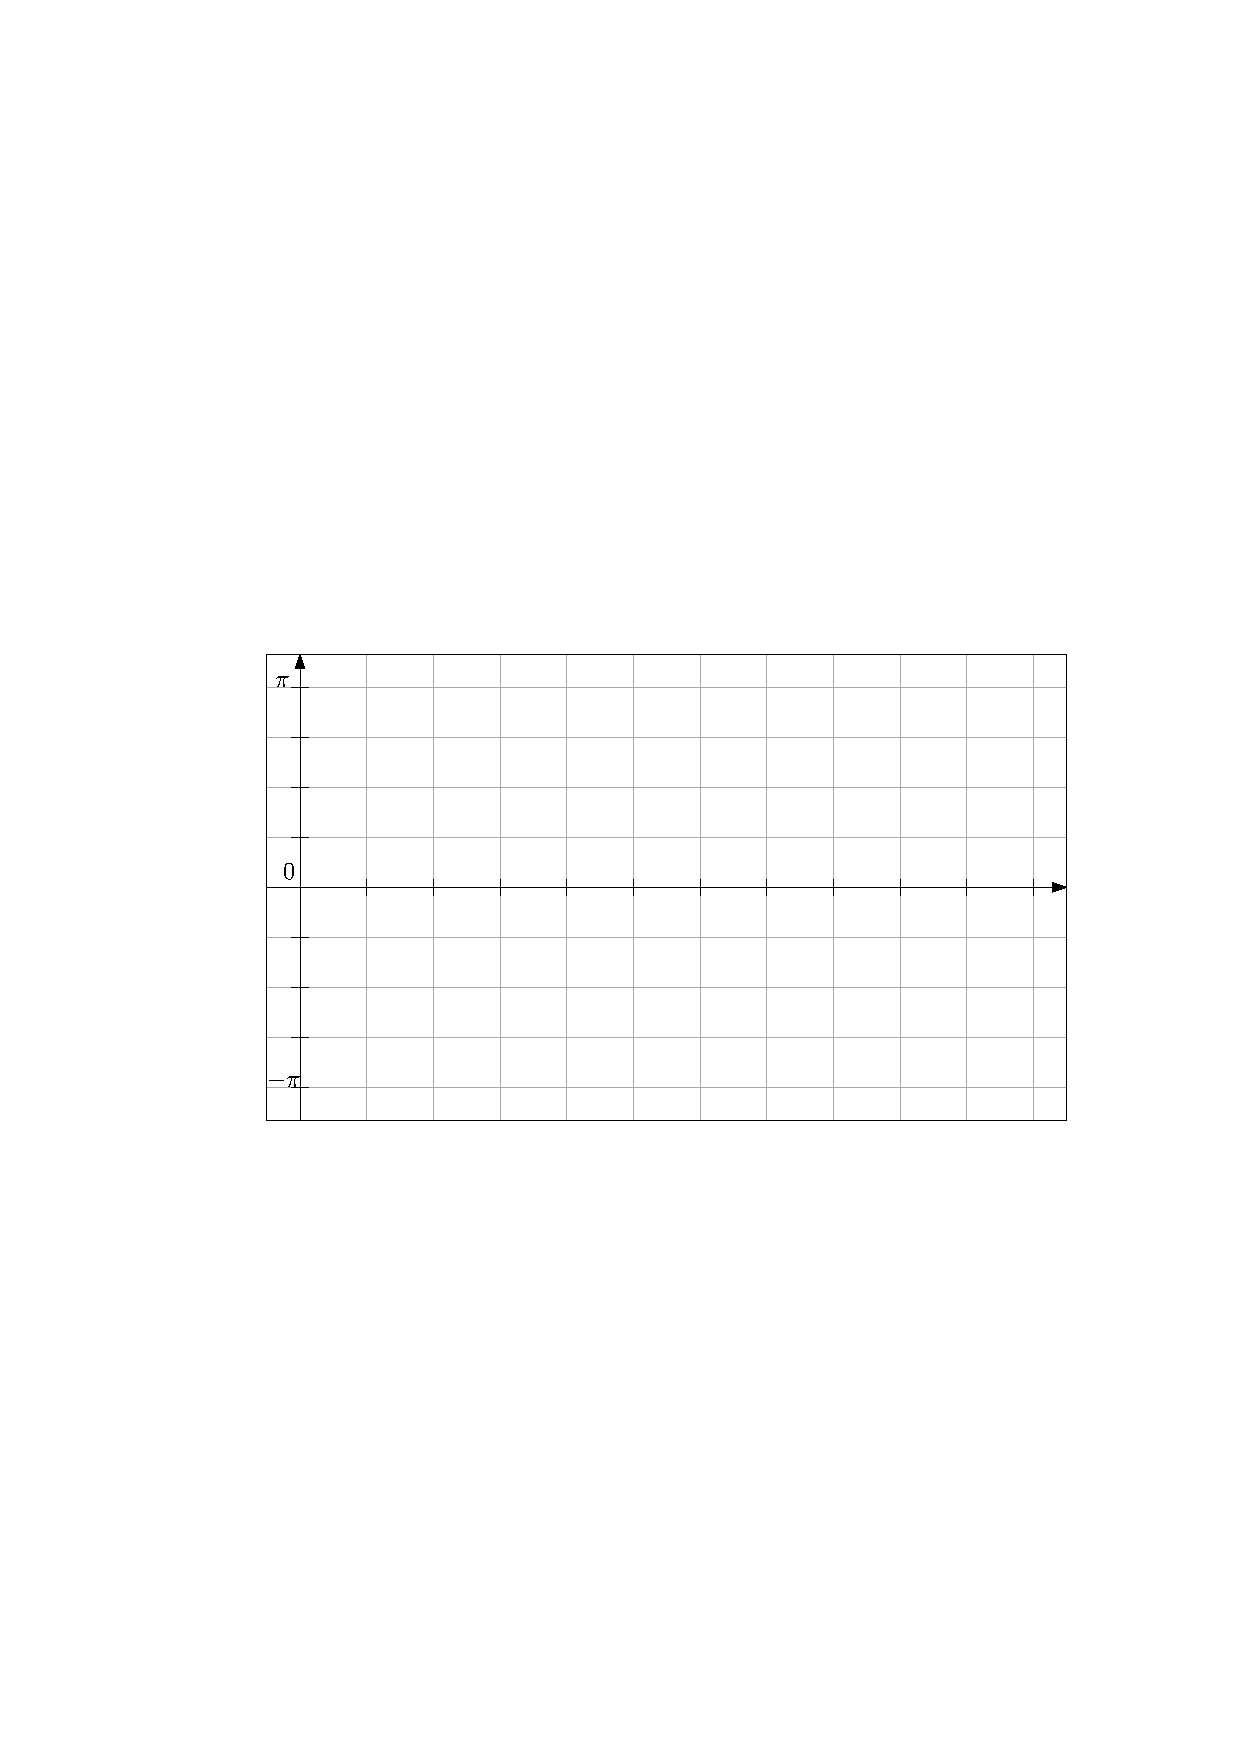
\includegraphics[width=\linewidth]{sources/1/grille.pdf}
\end{figure}


\end{document}
